\chapter{Routing}

\section{Home preparation}
Two of the more used routing protocols are RIP and OSPF.
Find information about these two protocols and compare them.
Describe what is the format of a routing table and explain how each of the protocols work.

Read the following quick guide:
\url{www.jaumebarcelo.info/teaching/lxs/routing/GUIA_RAPIDA_CISCO_2010.pdf}

And download the router user manuals:
\url{
www.jaumebarcelo.info/teaching/lxs/routing/manuals_routers.rar
}
\section{First Session}

In this first session each group will work with a router. 
The goals of this session are:
\begin{itemize}
\item Getting familiar with the configuration method.
\item Configuring ethernet interfaces.
\item Observe the RIP protocol in action.
\item Save the configuration in an external TFTP server.
\end{itemize}

Before disconnecting the computer from the Internet, download the TFTP server.
\url{http://tftpd32.jounin.net/}
Save it to one of the computers that you will use to connect to the router.

The routers are connected among them using the Ethernet interfaces and forming a topology that you will have to find out.
Use the console to connect to the routers (Hyperterminal or putty, 9600 bps, COM6).
The escape keystroke to exit a ping in a router is Ctrl-Alt-6.

\subsection{Checking the router status}

Use the console to connect to your router and explore the following commands.
Prepare a summary of what you can see with each command.
\begin{itemize}
\item show version
\item show protocols
\item show interfaces
\item show processes
\item show mem
\item show ip route
\item show history
\end{itemize}

\subsection{Create a ``Running'' and ``Startup'' configuration}
Enter the ``privileged EXEC'' mode (enable, pass ``cisco'') and global configuration (conf term). 
Find the commands to:
\begin{itemize}
\item show and change the router name
\item debugging mode configuration
\item send pings from the router
\item activate ``fair queueing'' at the ethernet interfaces (Fa0/0).
\end{itemize}

Use the command ``show running-config'' from the privileged mode.
Save the current configuration to the startup configuration (copy running-config startup-config).

\subsection{IP addresses configuration}
Go to your physical router box and check which interfaces are visible.

Use the ``show interfaces'' command to see what interfaces are available in the router.
Fill in a table that includes
\begin{itemize}
\item Interface name
\item MTU
\item Bandwidth
\item Encapsulation protocol
\end{itemize}

Enter the Ethernet interface configuration mode with the command 
\begin{lstlisting}
# interface <interface name>
\end{lstlisting}
and set the IP address to 192.168.10.XX, where XX is your group ID plus 10.
Use a /24 netmask.

\begin{center}
\sffamily\small
\begin{tabular}{>{\columncolor{tablegray}}p{15cm}}
\rowcolor{tableheader}
\multicolumn{1}{>{\columncolor{tableorange}}l}{Question}\\
What is the command that you have used?\\
\hline
\end{tabular}
\end{center}

Use the command
\begin{lstlisting}
# show interfaces
\end{lstlisting}
to verify the IP address assignment, and enable it with the command
\begin{lstlisting}
# no shutdown
\end{lstlisting}

Verify the line status and the interface status using the command 
\begin{lstlisting}
# show protocols
\end{lstlisting}

Use the commands
\begin{lstlisting}
# show cdp neighbors
\end{lstlisting}
and
\begin{lstlisting}
# show cdp neighbors detail
\end{lstlisting}
to see the neighboring devices.

Write down the information received from the different interfaces.
\begin{itemize}
\item neighbor identifier
\item ip address
\item port
\end{itemize}

Use the ping command to test the connectivity to the other routers in the lab and write down the round-trip times and other results that you may consider relevant.

Find out which is the network topology and sketch it in a figure.

Use the ``telnet'' command to connect to the router.
\begin{center}
\sffamily\small
\begin{tabular}{>{\columncolor{tablegray}}p{15cm}}
\rowcolor{tableheader}
\multicolumn{1}{>{\columncolor{tableorange}}l}{Question}\\
Is it possible to remotely configure a router?\\
\hline
Is login and password required?\\
\hline
Does a console user notice that there is an ongoing telnet connection?\\
\hline
Use telnet to change a parameter of the router (e.g., the name) and verify the changes both using the console and the telnet connection. What happens?\\
\hline
\end{tabular}
\end{center}

Do messages appear on the console when changes are done over telnet? What information is included in these messages?\\

Logout the telnet session to the Cisco router.

\subsection{IP routing configuration}

In this exercise we will enable the RIP protocol and check the status of the routing table as well as the RIP transactions of each router.

Check whether IP routing is enabled using the command
\begin{lstlisting}
# show protocols
\end{lstlisting}

\begin{center}
\sffamily\small
\begin{tabular}{>{\columncolor{tablegray}}p{15cm}}
\rowcolor{tableheader}
\multicolumn{1}{>{\columncolor{tableorange}}l}{Question}\\
What is the status of IP routing?\\
\hline
\end{tabular}
\end{center}

Enter the global config mode and enter the submenu router.
\begin{center}
\sffamily\small
\begin{tabular}{>{\columncolor{tablegray}}p{15cm}}
\rowcolor{tableheader}
\multicolumn{1}{>{\columncolor{tableorange}}l}{Question}\\
What is the purpose of this submenu?\\
\hline
\end{tabular}
\end{center}

Use the ``?'' command the available routing protocols and write down the results.
Enter into the configuration of RIP.

Use the command 
\begin{lstlisting}
# network <your network>
\end{lstlisting}
to associate your network to the RIP routing process.
Assume that we are working with ``C'' class addresses.
Therefore, the last byte of the network address must be 0.

Verify that the RIP protocol is now enabled and that your network has been recognized by the router using the command
\begin{lstlisting}
# show ip protocol
\end{lstlisting}
Observe the relevant parameters and answer the following questions:
\begin{center}
\sffamily\small
\begin{tabular}{>{\columncolor{tablegray}}p{15cm}}
\rowcolor{tableheader}
\multicolumn{1}{>{\columncolor{tableorange}}l}{Question}\\
What is the use of the timers?\\
\hline
What are their values?\\
\hline
Are they too small, or too large?\\
\hline
What happens if we change the values?\\
\hline
\end{tabular}
\end{center}

Verify the status of the routing table with the command
\begin{lstlisting}
# show ip route
\end{lstlisting}

\begin{center}
\sffamily\small
\begin{tabular}{>{\columncolor{tablegray}}p{15cm}}
\rowcolor{tableheader}
\multicolumn{1}{>{\columncolor{tableorange}}l}{Question}\\
What is the meaning of each of the fields in the table?\\
\hline
How can we check which are the networks to which RIP protocols is associated?\\
\hline
If there is no information, why?\\
\hline
\end{tabular}
\end{center}

Work together with another group to do this part.
If there is no other group ready, skip this exercise and move back to it when another group reaches this point.

Add an static route to the other group's network.
Use the ``ip route'' command from the configuration mode.
Explain what happens when you use ``traceroute'' to the other groups router (both interfaces).
Repeat the experiment after deleting the static route in one of the routers.
Explains what happens and why.

The command 
\begin{lstlisting}
# debug ip rip
\end{lstlisting}
shows the RIP messages that are sent and received by the router.
\begin{center}
\sffamily\small
\begin{tabular}{>{\columncolor{tablegray}}p{15cm}}
\rowcolor{tableheader}
\multicolumn{1}{>{\columncolor{tableorange}}l}{Question}\\
What are the source and destination of these packets?\\
\hline
What information do we obtain?\\
\hline
\end{tabular}
\end{center}

\subsection{Saving the router configuration in a TFTP server}

A convenient way to store a router's configuration is using TFTP.
We need to install the TFTP server in a PC with connectivity (ping connectivity) to the router.
Install the server and configure in which folder you want to save the router's configuration.

In the router, execute the command 
\begin{lstlisting}
# copy run tftp
\end{lstlisting}
and follow the instructions to enter the TFT server address (this is one of your PCs) and the filename that you want to use.
In the PC, open the configuration file using a text editor.
\begin{center}
\sffamily\small
\begin{tabular}{>{\columncolor{tablegray}}p{15cm}}
\rowcolor{tableheader}
\multicolumn{1}{>{\columncolor{tableorange}}l}{Question}\\
What can you observe?\\
\hline
\end{tabular}
\end{center}

Two copy the configuration in the TFTP server to the router, there are two different options.
Either use the command
\begin{lstlisting}
# copy tftp run
\end{lstlisting}
on the server or simply copy\&paste on the configuration terminal.

\section{Router Interconnection}
In this session, we will use the WAN (serial) interfaces of the routers.
The topology of the network is unknown to us and we have to figure it out.
In the previous session we used the ethernet interfaces to connect the routers, and in this session we will use the serial interfaces.

\subsection{Shutdown Ethernet interfaces}

Make sure that there is no cable connected to the ethernet interface, and that there is a cable connecting the serial interfaces.
Delete the IP address of the ethernet interface
\begin{lstlisting}
# no ip address
\end{lstlisting}
and administratively shutdown the interface
\begin{lstlisting}
# shutdown
\end{lstlisting}

Verify that the changes have been applied using
\begin{lstlisting}
# show run
\end{lstlisting}

\subsection{Configuration of the WAN serial interface}

From the privileged EXEC mode of your router, enter the global configuration mode.
Enter into the configuration of the WAN serial interface and configure it with the IP indicated on the blackboard.

The serial interfaces are interconnected by cables that, in the middle, have male/female connector.
The router in the female connector side sets the communication rate.
Use the command 
\begin{lstlisting}
# clock rate 12600
\end{lstlisting}
or the closest available rate.

Verify the configuration and use the command
\begin{lstlisting}
# no shutdown 
\end{lstlisting}
at both ends of the connection to enable the communication.
Then use the command
\begin{lstlisting}
# show protocols
\end{lstlisting}
to verify the state of the line.

Now we will gather information about neighbouring devices using the command
\begin{lstlisting}
# show cdp neighbours
\end{lstlisting}
or 
\begin{lstlisting}
# show cdp neighbours detail
\end{lstlisting}
and we will elaborate a table indicating, for each neighbour, the following information:
\begin{itemize}
\item Neighbour identifier
\item Neighbour IP address
\item Port
\end{itemize}

Make sure that routing is enabled using the following commands
\begin{lstlisting}
# ip routing
# router rip
# network 192.168.XX.0
\end{lstlisting}
and look at the routing tables using the command 
\begin{lstlisting}
# show ip route
\end{lstlisting}

Compare the routing tables to the ones obtained in the previous session and highlight the differences.

Send pings to the other devices in the network.
\begin{center}
\sffamily\small
\begin{tabular}{>{\columncolor{tablegray}}p{15cm}}
\rowcolor{tableheader}
\multicolumn{1}{>{\columncolor{tableorange}}l}{Question}\\
Which ones are reachable?\\
\hline
Which ones are not?\\
\hline
Why?\\
\hline
Are there differences in the round-trip-time compared to the measures taken in the previous session?\\
\hline
Why?\\
\hline
\end{tabular}
\end{center}

\subsection{Network Topology}
Prepare a sketch of the network topology that we have used in this session.

\begin{center}
\sffamily\small
\begin{tabular}{>{\columncolor{tablegray}}p{15cm}}
\rowcolor{tableheader}
\multicolumn{1}{>{\columncolor{tableorange}}l}{Question}\\
What are the differences?\\
\hline
What are the advantages?\\
\hline
And disadvantages?\\
\hline
\end{tabular}
\end{center}

\section{Configuration of an L2-L3 network}
This third session extends the previous one by including switches to the network topology.
The topology consists of a ring of routers connected in a ring using the serial interfaces.
Each router is connected using the ethernet interface to a local area network with two or more computers.
The devices used in this assignment are
\begin{itemize}
\item PCs
\item Six Cisco routers with an ethernet interface and two serial interfaces.
\item Three Cisco switches
\item Direct and cross-over RJ-45 cables.
\end{itemize}

\begin{figure}
\centering
\ifpdf
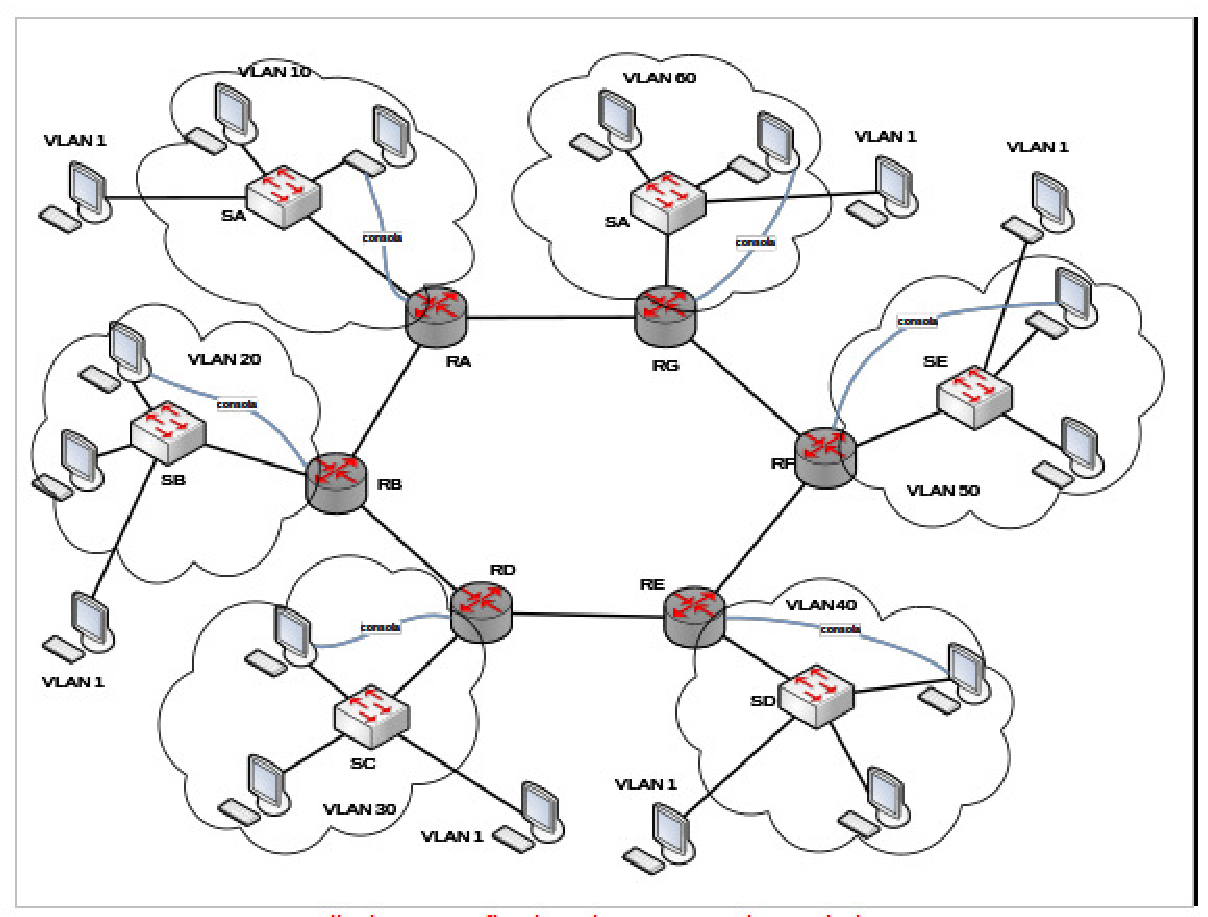
\includegraphics[width=0.9\linewidth]{Figures/routers_and_switches.pdf}
\else
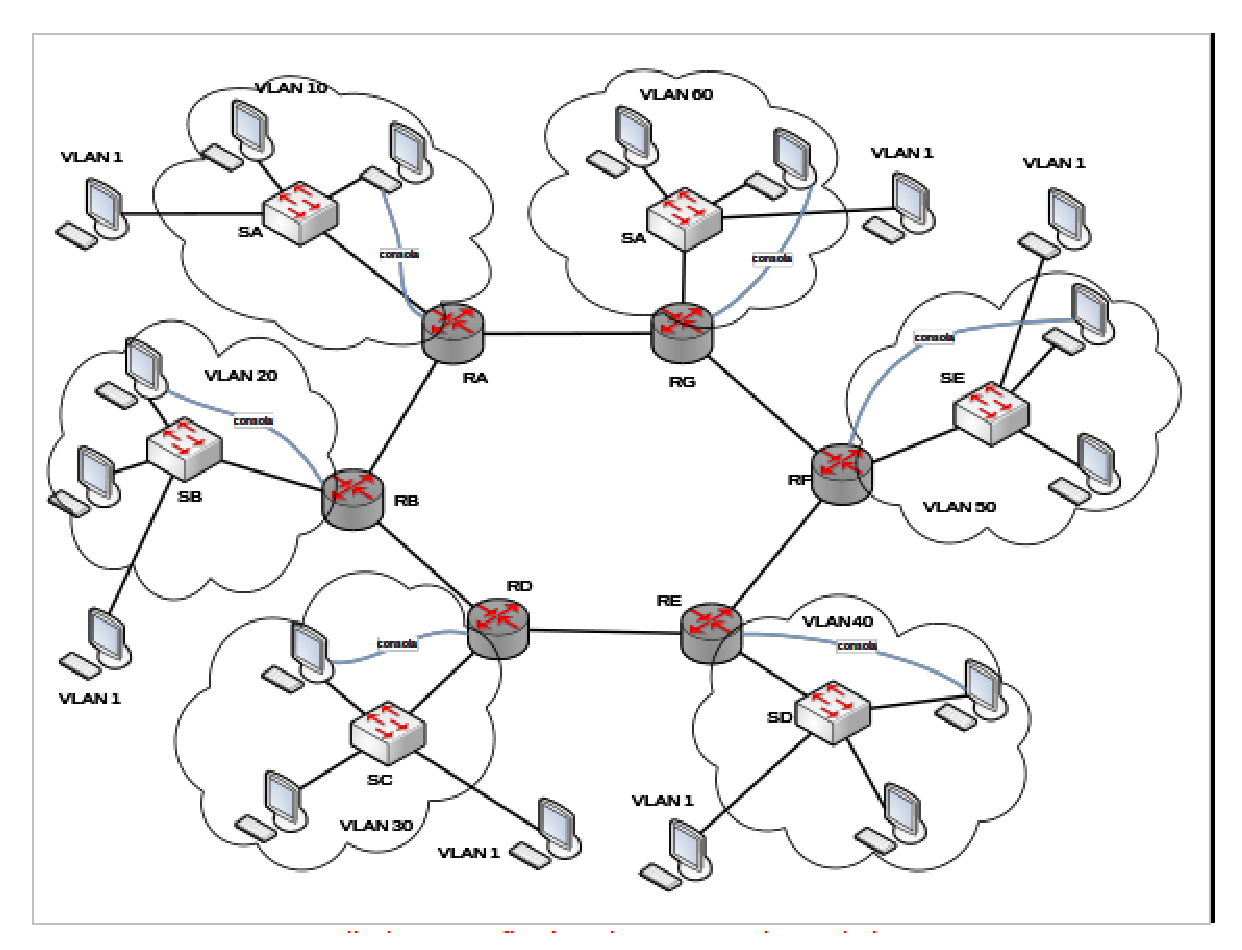
\includegraphics[width=0.9\linewidth]{Figures/routers_and_switches.eps}
\fi
\caption{Network topology that includes routers and switches}
\label{fig:StpTopology}
\end{figure}

Each group has to configure its router and its VLAN.
It is assumed that the previous session has been successfully completed and the connectivity tests were satisfactory.

\subsection{VLAN configuration}
We \texttt{telnet} our switch and enter the privileged EXEC mode.
Create a VLAN with a number equal to ten times your group number (group*10, e.g. VLAN 20 for group 2).
Assign a port connected to the router and one or two other ports connected to PCs. 
Remember to keep the port of the computer you are using for managing the switch in VLAN 1.
Use an IP equal to 192.168.1.XX where XX is the group multiplied by ten for the computer in VLAN 1.
Use an IP 192.168.VLAN.YY for the other VLAN. 
YY is going to be 1 for the router and 2 for the computer.
You can use YY equal to 3 if you have another computer.

Test the connectivity between your different computers and with computers of other groups.
Write down when the \texttt{ping} work and when it does not work and provide an explanation.

\subsection{Configuring the Router LAN interface}

In the router console enter the privileged EXEC mode and use the command 
\begin{lstlisting}
# show interfaces
\end{lstlisting}
to see the interfaces which are available in the router.
We enter the global configuration mode and thin in the configuration of the LAN (ethernet) interface.
We configure the IP for this interface.
Then we enable the interface
\begin{lstlisting}
# no shutdown
\end{lstlisting}
and check the link status led.
We can also check the status of the line and the interface using the command
\begin{lstlisting}
# show protocols
\end{lstlisting}

Let's enable routing.
From the global configuration menu we enter the router menu and we use the command
\begin{lstlisting}
# network 192.168.VLAN.0
\end{lstlisting}
to associate our network to the routing process.
We will assume that we are using class C networks.
Then we use the command
\begin{lstlisting}
# show routes
\end{lstlisting}
To see the routing tables.

\subsection{Connectivity test}

We add our router's IP as as the default GW for our PC connected to the router.
We perform ping tests from the router to the other devices of the network.
Finally, we fill in a table with the following information:
\begin{itemize}
\item destination IP
\item packet loss
\item average delay
\end{itemize}

Now we repeat the tests from the computer.
If we are on a linux box, try also tracepath and mtr.

We will include the configuration of the switch and the router in the  lab assignment report.

